\setAuthor{Jaan Kalda}
\setRound{piirkonnavoor}
\setYear{2022}
\setNumber{G 10}
\setDifficulty{10}
\setTopic{TODO}

\prob{Pingpong}
Juuresoleval graafikul (suuremalt lisalehel) on toodud heli intensiivsus (detsibellides) funktsioonina ajast, kui pingpongipall põrkab üles-alla vastu horisontaalset lauda. Heli tugevuse andmepunktid on võetud ligikaudu iga \num{0.1} sekundi järel. Leidke graafikut kasutades nii täpselt kui võimalik, mitu protsenti palli kineetilisest energiast muundub iga põrke ajal soojuseks\\
\osa esimeste põrgete ja \\
\osa viimaste põrgete jaoks.\\
Pidage silmas, et see protsent püsib enam-vähem konstantne esimesest kuni viienda põrkeni ning samuti alates kolmeteistkümnendast põrkest kuni põrkumiste lõpuni.
\begin{figure}[!h]
  \centering
  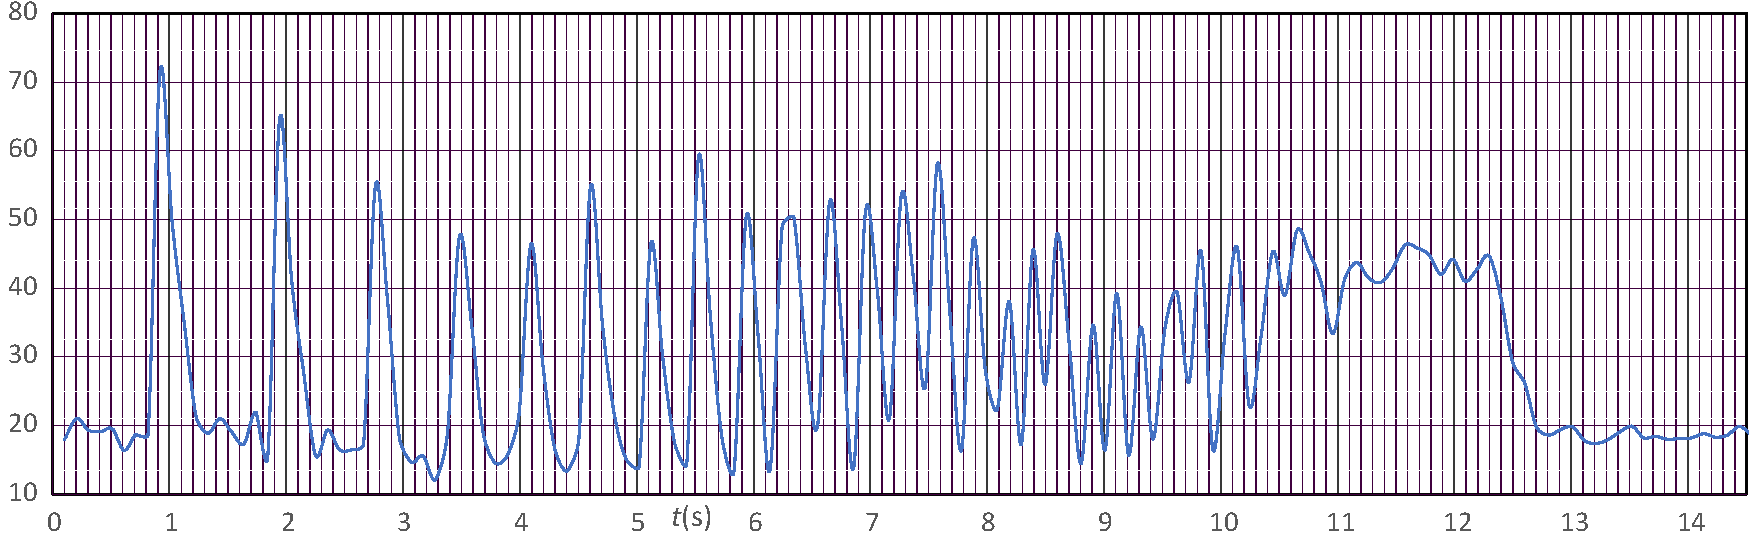
\includegraphics[width=\textwidth]{2022-v2g-10-yl.pdf}
\end{figure}


\hint

\solu
\emph{Märkus}: graafikult numbrite välja lugemise eest antakse punkte isegi siis, kui õpilane ei oska nendega midagi peale hakata.

\osa Teeme kindlaks esimese kuue põrke hetked sekundites: \num{0,92}; \num{1,93}; \num{2,78}; \num{3,49}; \num{4,1}; \num{4.61} (\p1; punkti teenimiseks piisab, kui välja on loetud esimesed kaks ja viimased kaks andmepunkti; kui on välja loetud vähem, kui neli andmepunkti, siis punkte ei anta; kui välja loetud andmepunktid ei sisalda esimest või kuuendat põrget, siis antakse \p{0,5}). Kuigi samplimise sagedus on $\SI{0.1}s$, siis graafikult on näha, et tulemusi saab välja lugeda täpsemalt --- ilmselt on graafikuid interpoleeritud (seda hindamisskeem ka eeldab: punkte ei alandata, kui välja loetud arvväärtused erinevad eeltoodutest mitte rohkem, kui $\SI{0.02}s$ võrra; kui ühes andmepunktis on suurem viga, mis pole siiski rohkem, kui  $\SI {0.04}s$, siis alandatakse skoori \p{0,5} võrra ja kui vigade arv on suurem, siis punkte ei anta).

Nende põhjal saame arvutada esimesele viiele põrkele järgnenud lennuajad sekundites: \num{1,01}; \num{0,85}; \num{0,71}; \num{0,61}; \num{0,51} (\p1; kui esimeses või viimases arvus on viga suurem, kui $\SI {0.03}s$, siis alandatakse skoori \p{0,5} võrra ja kui see on suurem, kui $\SI{0.05}s$, siis punkte ei anta).

Ülesande eelduste kohaselt peaks vähenema kineetiline energia geomeetrilise jadana: $T_n=mv_n^2/2=T_0k^n$ (valemina kirja panemise eest \p1). Kiirus $v_n$ on võrdeline ruutjuurega energiast, seega $v_n=v_0\sqrt{k^n}$ \p1 ning lennuaeg $t_n=2v_n/g$ on võrdeline kiirusega, seega $t_n=t_0\sqrt{k^n}$ \p1. Mõõdetud andmete kasutamise parim meetod oleks kanda need graafikule, kus horisontaalteljel on põrkenumber ja vertikaalteljel --- lennuaja logaritm $\ln t_n=\ln t_0 + \frac 12n\ln k$:  ning nimetatud teljestikus peaks tulema sirgjoon, mille kahekordne tõusunurga tangens annaks meile $\ln k$ väärtuse. Aga hea tulemuse saame ka, kui võtame viienda ja esimese lennuaja suhtest ruutjuure:  $k=\sqrt{0.51/1.01}\approx 0.71$, mis tähendab, et 29\% kineetilisest energiast kaob igal põrkel (ükskõik kumma meetodi rakendamine annab \p1). Õige numbrilise vastuse eest (vahemikus 25\% kuni 35\%) saab \p1, ebatäpse vastuse eest (vahemikus 20\% kuni 40\%) saab pooled punktid, st \p{0,5}. NB! Arvulise väärtuse eest saab punkte vaid siis, kui see tuleneb õige meetodi rakendamisest.

\osa Alates üheksandast põrkest on põrkeajad nii väiksed, et eelpooltoodud arvutuste läbiviimine on küll võimalik, kuid ebatäpne; kui viiakse läbi selline analüüs, siis saab selle ülesande osa (b) eest vaid kuni \p2: vastuse eest vastavalt allpooltoodud reeglile kuni \p1 ning kuni \p1 graafikult põrkehetkede välja lugemise eest (kui kasvõi ühes arvutusteks vajalikus andmes on viga suurem, kui $\SI{0.02}s$, siis \p{0,5} ning kui see on suurem, kui $\SI{0.04}s$, siis \p0).

Selle asemel kasutame teist meetodit: kuivõrd põrkeaegadest moodustub geomeetriline jada, siis palli seismajäämise hetke saab avaldada geomeetrilise jada summana. Kaheteistkümnes põrge toimub ajahetkel $\SI{6.97}s$ ja järgmine põrge --- ajahetkel $\SI{7.27}s$ (mõlemad andmepunktid kokku \p1; kui kasvõi ühes neist on viga suurem, kui $\SI {0.02}s$, siis alandatakse skoori \p{0,5} võrra ja kui see on suurem, kui $\SI {0.04}s$, siis punkte ei anta) ning põrked lõppevad ajahetkel $\SI{12.3}s$ (\p1; kui viga on suurem, kui $\SI {0.02}s$, siis alandatakse skoori \p{0,5} võrra ja kui see on suurem, kui $\SI {0.04}s$, siis punkte ei anta). Siit saame leida kaheteistkümnenda põrke kestvuse $t_{12}=\SI{0.3}s$.
Mõõtes nüüd ajavahemiku kaheteistkümnendast põrkest põrkumiste lõpuni $T=t_{12}/(1-\sqrt k)=\SI{5.33}s$ \p1 on lihtne leida $k=(1-t_{12}/T)^2\approx 0.88$ \p1, mis tähendab, et igal põrkel kaob 12\% kineetilisest energiat \p1. Kui vastus erineb antud numbrist rohkem, kui 1\% võrra, siis saab numbrilise vastuse eest vaid \p{0,5} punkti ning kui see erineb rohkem, kui 2\% võrra, siis punkte ei saa.

\emph{Märkus:} Tasub tähele panna, et saadud tulemus pole väga täpne, sest samplimise sagedus on ju vaid $\SI{0.1}s$, mistõttu $t_{12}$ leidmise suhteline viga on võrdlemisi suur. Seetõttu on täpsemateks arvutusteks vaja kasutada ka järgnevaid andmepunkte (põrgete hetked $\SI{7.58}s$, $\SI{7.88}s$, $\SI{8.17}s$ ja $\SI{8.39}s$) ning keskmistada. Geomeetrilises jadas on jada keskmine liige kõigi liikmete geomeetriline keskmine, aga kui keskmistatavad arvud erinevad üksteisest vähe, siis on geomeetriline keskmine ligikaudu võrdne aritmeetilise keskmisega. Seega me võime leida $t_{14}=(\num{8.39}-\num{6.97})\unit{s}/5= \SI{0.284}s$. Arvutades nüüd juba ajavahemiku neljateistkümnendast põrkest põrkumiste lõpuni $T'=t_{14}/(1-\sqrt k)=\SI{4.72}s$, saame tulemuseks $k=(1-t_{14}/T')^2\approx 0.88$, mis osutus võrdseks me esialgse tulemusega.
\probend